Proteins are large biomolecules formed by one or more chains of amino acids.
The genetic information contained in the DNA only specifies the sequence of these amino acids, the so-called \emph{primary structure} of the protein.
It has been experimentally observed that purified proteins, i.e. proteins purified away from other cellular components, tends to spontaneously refold after being completely unfolded \cite{ProteinFolding1990}.
Understanding why and how protein folds may be a vital task for biological researches.
In fact, in order to be biologically active, a protein must adopt specific folded three-dimensional structures.
The main observable to look for in order to extract some information about protein folding is the free energy of the protein itself.
We can distinguish between three main conformational states of a protein.

\subsection{Unfolded state}
The first state we're going to discuss is the \emph{unfolded} state.
The ideal unfolded protein is the random coil, where all conformations have comparable free energies except when atoms of the polypeptide chain come into proximity.
The number of possible conformations for a protein grows exponentially with its length: it would therefore be impossible for a fully unfolded protein to encounter on a finite timescale all its possible conformations.
Consequently, the native conformation is unlikely to be found by a totally random process.

\subsection{Intermediate state}
It has been experimentally observed that many proteins exist, under certain conditions, in stable conformations that are not completely folded nor completely unfolded.
This may be caused by the free-energy landscape of the protein itself, that contains many local minima, as we can see from Fig. \ref{fig:energy_landscape}.

\begin{figure}[H]
    \centering
    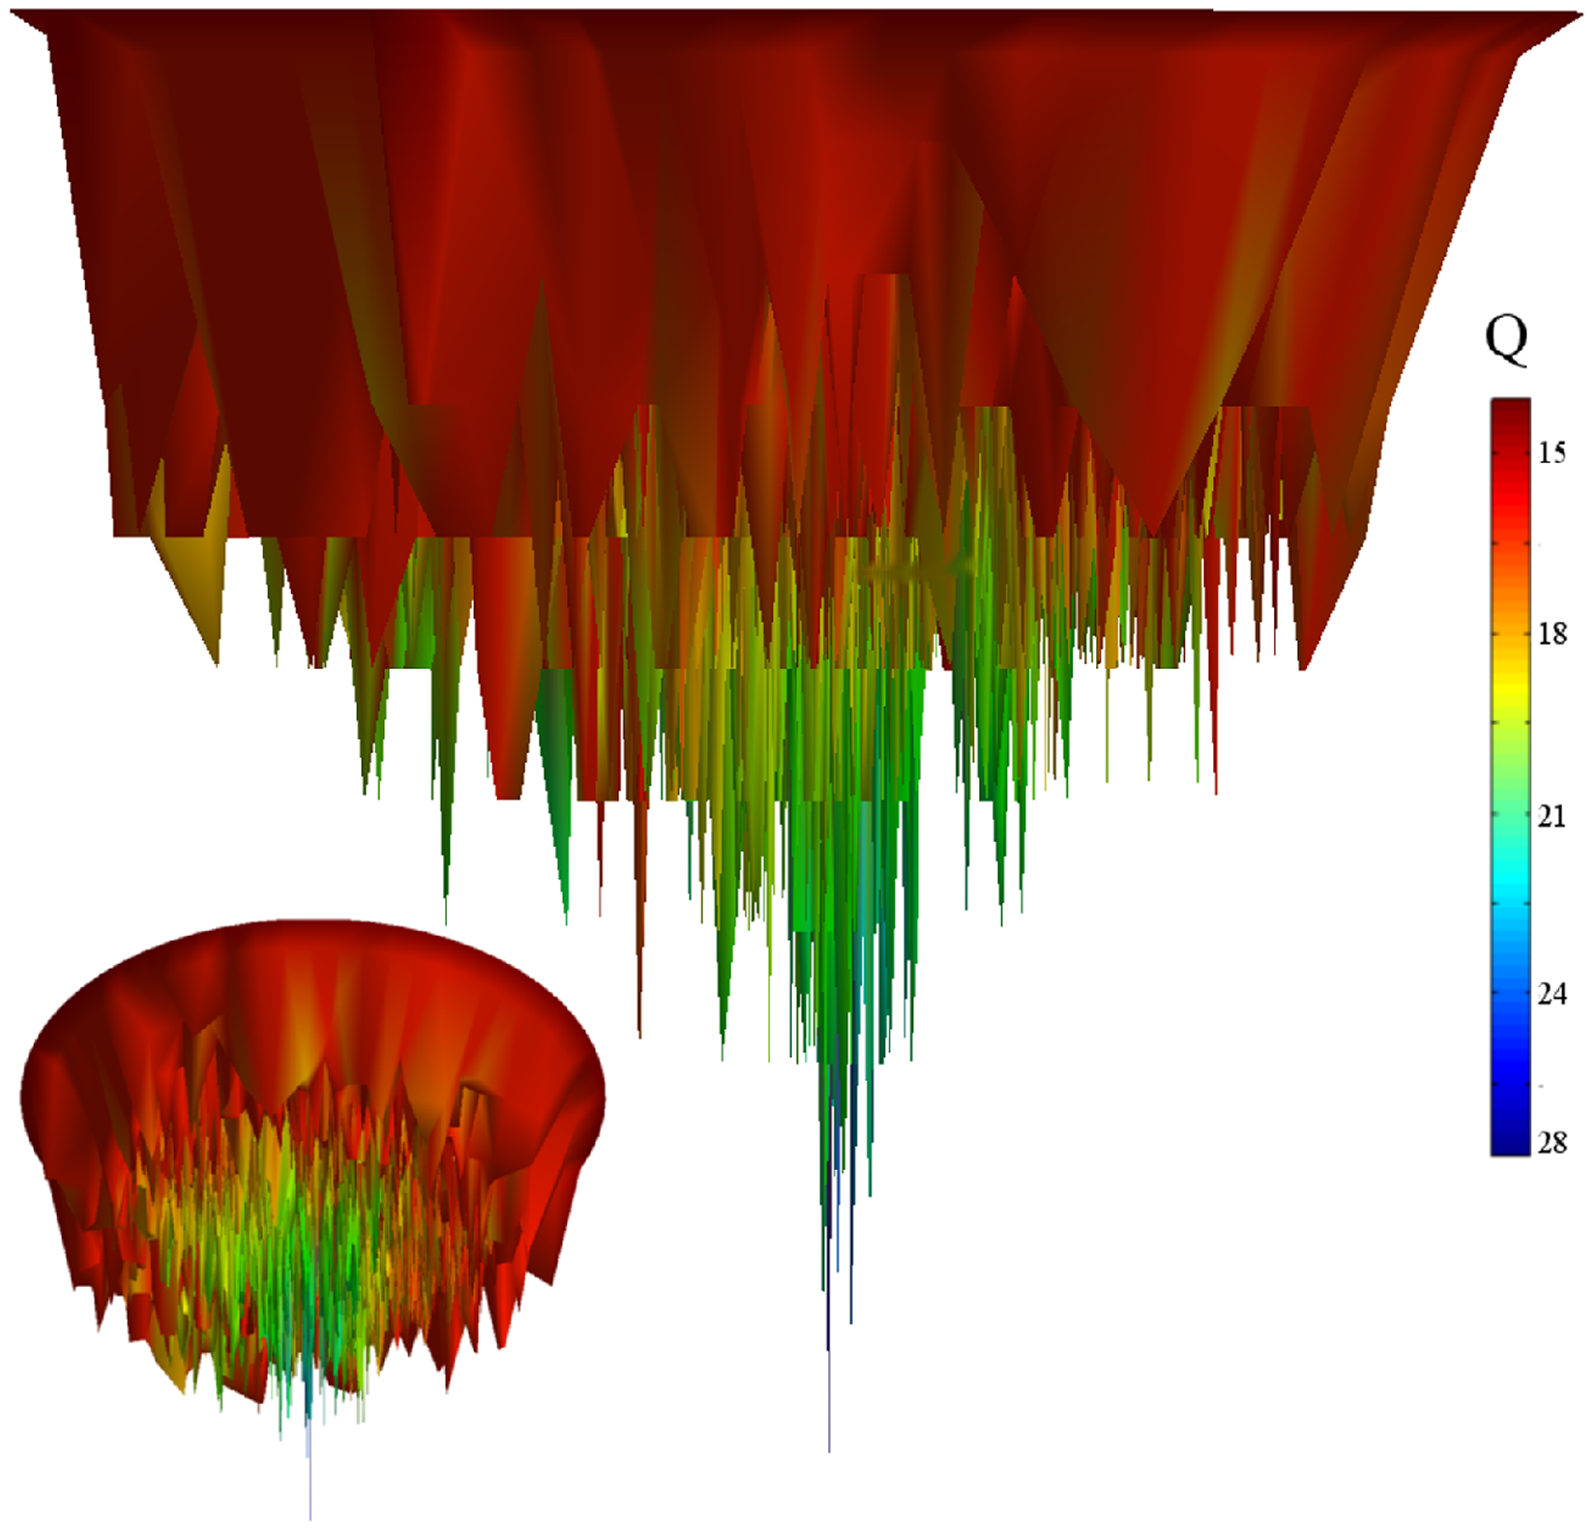
\includegraphics[width=.75\textwidth]{./img/energy_landscape.png}
    \caption{\emph{Example of a protein's energy landscape taken from \cite{energyLandscape}.
                The third axis (depth) of the funnel is associated with the energy of the local minima, and the color map represents the reaction coordinate Q.
                It's possible to see a lot of minima that are not the global one.}}
    \label{fig:energy_landscape}
\end{figure}

\subsection{Native state}
We call \emph{native} state the conformational state in which the protein is fully folded, i.e. in its free-energy minimum.
The native conformations of proteins are known in great detail from the structures determined by X-ray crystallography.
How much alteration is necessary before a protein no longer folds to its normal conformation, either remaining unfolded or in an Intermediate state, is not certain.
Proteins have been found to be surprisingly adaptive to mutations that would be expected to be disruptive, but the hydrophobic core seems to be the most critical aspect for stability of the normal folded state.
This criticality is the basis of HP model that we'll discuss later.

\subsection{Stability of the folded state}
From a physical point of view we know that exists an equilibrium constant $k_{eq} = \frac{\left[\text{N}\right]}{\left[\text{U}\right]}$ such that the free energy at equilibrium is
\begin{equation*}
    \Delta G = G_{\text{N}} - G_{\text{U}} = k_BT\ln k_{eq}
\end{equation*}
The large heat capacity change upon protein unfolding causes there to be a temperature at which stability of the folded state is at a maximum: the stability of the folded state decreases at both higher and lower temperatures.
Despite this definition, it is clear that the folding problem has an aspect more similar to
\begin{equation*}
    \text{U} \leftarrow fast \rightarrow \text{I} \leftarrow slow \rightarrow \text{N}
\end{equation*}
where we've also to consider the intermediate state.